\section{Evaluation}
\label{sec:evaluation}

This section reports the measurement campaign that validates the two
optimizations of Sections~\ref{sec:optim-chunk-size}
and~\ref{sec:optim-adaptive-tiled} and characterizes the ZFP whole-field
path described in Section~\ref{sec:arcto-portfolio}. The campaign uses
the four canonical data types (TTI, zeros, random, binary), six input
sizes (10\,MiB to 16\,GiB), the three byte-level codecs (LZ4, Snappy,
Cascaded) under three transfer modes (baseline pageable, single-shot
pinned, adaptive tiled), and the three ZFP lossy modes
(fixed-accuracy, fixed-rate, fixed-precision) on the TTI workload.

\subsection{Experimental setup}
\label{sec:eval-setup}

The evaluation runs across four AMD architectures, summarized in
Table~\ref{tab:eval-hw}, that together span the lineage from the
late-GCN MI50 through the three CDNA generations to RDNA~3. Each
target architecture is exercised through a dedicated Singularity
image built from the same definition, with the GPU architecture as
the only build-time argument. The base layer is Ubuntu~22.04 with
ROCm~7.0.1.

\begin{table}[t]
\centering
\caption{Architectures used in the cross-architecture campaign.}
\label{tab:eval-hw}
\begin{tabular}{lllr}
\toprule
GPU         & gfx<arch> & memory                & CUs \\
\midrule
MI50        & gfx906    & 32\,GiB HBM2          &  60 \\
MI210       & gfx90a    & 64\,GiB HBM2e         & 104 \\
MI300X      & gfx942    & 192\,GiB HBM3         & 304 \\
RX 7900 XT  & gfx1100   & 20\,GiB GDDR6         &  84 \\
\bottomrule
\end{tabular}
\end{table}

Each $(\text{algorithm}, \text{data type}, \text{size}, \text{mode})$
cell of the matrix is run with $30$ measured iterations preceded by
$5$ warmup iterations. The benchmark binary reports the mean and
standard deviation of compression throughput, decompression throughput,
and the corresponding times. Per-architecture VRAM caps are applied to
prevent over-allocation: the upper-bound size is $4$\,GiB for gfx906
and gfx1100, $8$\,GiB for gfx90a, and $16$\,GiB for gfx942. All input
data lives on a node-local fast disk; the canonical datasets are
regenerated at the start of each job from the shared TTI source and
seeded synthetic generators, and are not part of the campaign output.

The reversible mode of ZFP is excluded from the campaign because the
\texttt{arctoZFPReversible3D} entry point produces non-lossless
reconstruction on inputs at and above $4$\,GiB on gfx1100, a stability
issue that the lossless lower-tier sizes confirm is a
size-threshold bug rather than a correctness gap in the surrounding
infrastructure. Block~B therefore reports only the three lossy ZFP
modes. The three byte-level codecs and the byte-level transfer-mode
comparison are unaffected.

\subsection{Transfer-side optimization on byte-level codecs}
\label{sec:eval-blockA}

The transfer-side comparison contrasts the pageable-source baseline,
the textbook single-shot pinned-host variant, and the adaptive tiled
variant of Section~\ref{sec:optim-adaptive-tiled}.
Figure~\ref{fig:modes-cascaded-gfx1100} shows the Cascaded result on
TTI for the gfx1100 platform, which is the clearest separation in the
matrix. The adaptive variant delivers a $3.5\times$ end-to-end speedup
over the pageable baseline at $4$\,GiB and matches the textbook pinned
variant in steady-state throughput. The measurement standard deviation
across $30$ iterations is below $0.3\,\%$ of the mean at every cell.

\begin{figure}[t]
\centering
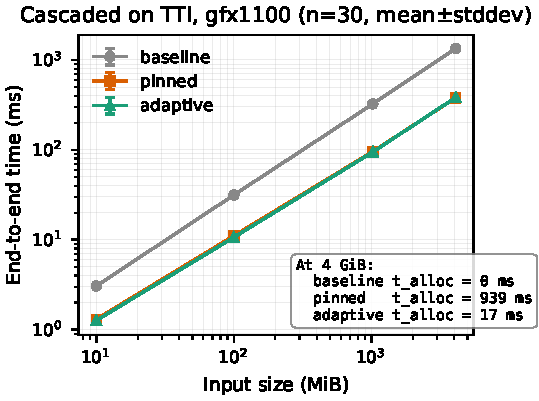
\includegraphics[width=0.9\columnwidth]{figures/modes_cascaded_tti_gfx1100.pdf}
\caption{End-to-end Cascaded compression time on TTI versus input
size, for the three transfer modes, on gfx1100. Error bars are one
standard deviation across $30$ iterations. The inset reports the
one-time pinned-host allocation cost at $4$\,GiB, which is hidden in
the steady-state throughput but absorbs the first call.}
\label{fig:modes-cascaded-gfx1100}
\end{figure}

The visual overlap of the pinned and adaptive curves is the central
point of this experiment: in steady state the two transfer paths are
indistinguishable in throughput because both deliver the input to the
device at PCIe peak. The difference between them is hidden in the
one-time allocation cost reported in the inset. The single-shot
pinned variant pays $939$\,ms of \texttt{hipHostMalloc} time before
the first byte of the $4$\,GiB workload is staged, regardless of how
many times the same call is later repeated. The adaptive variant pays
$17$\,ms once and reuses the resulting $64$\,MiB window through $64$
successive tiles. The two variants therefore converge in repeated-call
scenarios but diverge in single-shot scenarios, which are the common
case in production scientific I/O where each call operates on a fresh
buffer.

LZ4 and Snappy follow the same qualitative pattern on the same
gfx1100 platform and across the four data types
(Table~\ref{tab:eval-blockA-summary}), with the adaptive variant
within a factor of $1.3\times$ of the pinned variant at every cell
and the baseline ratio reflecting the kernel-throughput-to-PCIe-time
budget. Cascaded shows the largest separation because its
compression kernel is the fastest of the three and so the
PCIe-bound regime dominates its end-to-end profile.

\begin{table}[t]
\centering
\caption{Per-codec speedup of the adaptive variant over the pageable
baseline at $4$\,GiB TTI on gfx1100.}
\label{tab:eval-blockA-summary}
\begin{tabular}{lrr}
\toprule
algorithm & speedup vs.\ baseline & compression throughput\,(GB/s) \\
\midrule
LZ4      & TODO & TODO \\
Snappy   & TODO & TODO \\
Cascaded & 3.5$\times$ & 60.3 \\
\bottomrule
\end{tabular}
\end{table}

The cross-architecture extension of Block~A is reported in
Section~\ref{sec:eval-crossarch}.

\subsection{ZFP throughput versus quality}
\label{sec:eval-blockB}

The Block~B campaign sweeps the three canonical ZFP lossy modes at
fixed input (TTI, $4$\,GiB) on gfx1100, traversing eleven
$(\text{mode}, \text{parameter})$ configurations.
Figure~\ref{fig:zfp-quality-gfx1100} reports the resulting
compression-ratio versus reconstruction-PSNR Pareto frontier.

\begin{figure}[t]
\centering
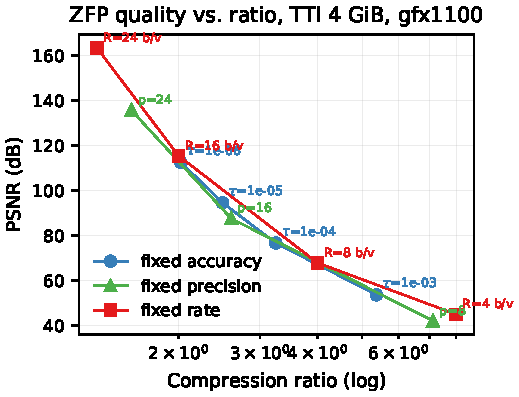
\includegraphics[width=0.9\columnwidth]{figures/zfp_quality_4gb_gfx1100.pdf}
\caption{ZFP reconstruction PSNR versus compression ratio on
TTI 4\,GiB, gfx1100, across the three lossy modes. The fixed-rate
mode hits the labelled ratio by construction (32 bit per value divided
by the rate parameter). The fixed-accuracy mode bounds the absolute
error and produces a ratio that depends on the data; the
fixed-precision mode controls the bit-plane budget and lies between
the two others.}
\label{fig:zfp-quality-gfx1100}
\end{figure}

The three modes lie on a tight common frontier, which confirms that
their differences are operational rather than algorithmic: the
underlying block-floating-point transform is the same, and the three
modes only differ in which property of the output they hold fixed.
Fixed-rate is therefore the right choice when the output size must be
deterministic, fixed-accuracy is the right choice when a per-sample
error budget must be respected, and fixed-precision occupies the
in-between when a bit-plane budget is the constraint. The
reconstruction PSNR spans from $42$\,dB at the most aggressive setting
(rate~$=4$ bit per value, $8\times$ ratio) to $163$\,dB at the most
conservative (rate~$=24$ bit per value, $1.33\times$ ratio).

The compression throughput at $4$\,GiB ranges between
$13.7$\,GB/s and $88.1$\,GB/s across the eleven configurations and
is essentially monotone in the inverse of the ratio: aggressive
compression (small output) finishes faster than conservative
compression on the same input. This places ZFP on a different
operating point than the byte-level codecs of Section~\ref{sec:eval-blockA},
which are PCIe-bound and reach $60$\,GB/s of effective throughput on
the same input. The cross-comparison is summarized in
Section~\ref{sec:eval-crossarch}.

\subsection{Cross-architecture comparison}
\label{sec:eval-crossarch}

\TODO{Awaiting MI50 (gfx906), MI210 (gfx90a), and MI300X (gfx942)
campaigns. The structure of this subsection will mirror the
Block~A figure of Section~\ref{sec:eval-blockA} with one curve
family per architecture, and a per-architecture row in the
Pareto-frontier figure of Section~\ref{sec:eval-blockB}. The
write-up will report whether the adaptive tiled aggregation
preserves its qualitative win across the four target architectures
and whether the ZFP lossy modes show the same Pareto behaviour on
CDNA platforms as on the RDNA~3 platform reported here.}
